\documentclass[uct_visualisation_thesis.tex]{subfiles}

Aplikacja jest podzielona na pięć oddzielnych modułów: \textit{Algorytm}, \textit{Serializacja}, \textit{Wizualizacja} i \textit{Gry}, które będą funkcjonować w obrębie nadrzędnego modułu -- \textit{Aplikacji głównej}. Cele każdego z modułów i zadania powierzone im są przedstawione w rozdziałach \ref{subsec:algorithm} - \ref{subsec:mainapp}.

\section{Wykorzystane technologie}
W naszym projekcie zdecydowaliśmy się skorzystać z technologii wymienionych poniżej.
\begin{enumerate}
	\item Języka \textit{Python} w wersji 3.7.2, który jest udostępniany na licencji \textit{GNU General Public License}.
	\item Biblioteki \textit{VisPy} w wersji 0.6.3, która udostępnia komponenty związane z wizualizacją graficzną. Wykorzystujemy tę bibliotekę w połączeniu z \textit{OpenGL} w wersji 2.1. Biblioteka \textit{VisPy} jest stworzona w oparciu o licencję \textit{BSD}, co w kontekście projektu na pracę inżynierską pozwala na modyfikowanie i wykorzystywanie jej.
	\item Biblioteki \textit{NumPy} w wersji  1.18.1, która odpowiada za wydajne operacje na macierzach. Zgodnie z umową licencyjną opisaną przez autorów \textit{NumPy}, można wykorzystywać ich narzędzie w zakresie pracy naukowej.
	\item Nakładki na bibliotekę \textit{Qt} -- \textit{PyQt} w wersji 5.9.2. \textit{PyQt} umożliwia tworzenie interfejsu graficznego. Dla projektów takich jak praca inżynierska, \textit{PyQt} dystrybuowana jest na zasadach \textit{GNU General Public License}.
	\item Biblioteki \textit{fman build system (fbs)} w wersji 0.8.4, ułatwiającej pakowanie aplikacji korzystających z biblioteki \textit{PyQt} w celu stworzenia pliku instalacyjnego. To oprogramowanie dystrybuowane jest na zasadach \textit{GNU General Public License}.
	\item Narzędzia \textit{pdoc} w wersji 0.3.2, służącego do automatycznego generowania dokumentacji aplikacji. Zgodnie z umową licencyjną opisaną przez autorów \textit{pdoc}, można wykorzystywać ich narzędzie bez ograniczeń.
\end{enumerate}


\section{Moduł -- Algorytm} \label{subsec:algorithm}
Moduł \textit{Algorytm} jest implementacją metody MCTS, korzystającą z wariantu UCT. Odpowiedzialnością tego modułu jest wyznaczanie kolejnego ruchu na podstawie dostarczonego stanu gry. Opisywany moduł będzie odpowiadał za iteracyjne tworzenie drzewa stanów i przeszukiwanie go w celu wyznaczenia najbardziej korzystnego ruchu. Użytkownik będzie miał możliwość zmiany liczby iteracji algorytmu albo ograniczenie czasowe jego działania.\\

W listingu \ref{lst:mcts} opisującym zaimplementowany algorytm operujemy na trzech istotnych zmiennych: \textit{tree}, \textit{curr\textunderscore node} i \textit{curr\textunderscore state}. Odpowiedzialnością struktury opisującej drzewo \textit{tree} jest przechowywanie korzenia oraz stanu wyjściowego rozgrywki, który jest tej samej struktury co zmienna \textit{curr\textunderscore state}. Struktura opisująca wierzchołek \textit{curr\textunderscore node} przechowuje wszystkie informacje na temat wierzchołka drzewa, wraz z referencjami do wierzchołków potomnych i rodzica. Dokładne relacje między komponentami zostały opisane na Rysunku \ref{rys:umldiagram_algorithm}.


\section{Ewaluacja rozgrywek}
Algorytm dla wygranych gier zwraca wartość $1$, dla remisów $0.5$, a dla przegranych $0$.
W celu usprawnienia działania algorytmu, do fazy symulacji została dodana funkcjonalność przerywania rozgrywanych gier po zadanej liczbie ruchów. Po przerwaniu symulacji w fazie propagacji wstecznej przekazana zostaje wartość nagrody wyznaczona przez pewną funkcję, która przyjmuje wartości z przedziału $[0.2, 0.8]$. Funkcja może przyjmować różne wartości, a jej najważniejszą cechą jest, że dla sytuacji neutralnej zwraca wartość $0.5$, tak jak w przypadku remisu.\\

W przypadku mankali za główny czynnik pozwalający określić wypłatę dla gracza przyjęta została różnica pomiędzy punktami tego gracza, a punktami jego przeciwnika. Maksymalną liczbą punktów do uzyskania jest $48$, a minimalną $0$, stąd zakres wypłat wynosi $[-48, 48]$. Zastosowano funkcję liniową, która dla różnicy punktów wynoszącej $0$ przyjmuje wartość $0.5$. Wzór funkcji został przedstawiony we wzorze \ref{formula:mancala}, a jej reprezentację graficzną można ujrzeć na wykresie \ref{rys:eval_mancala}.

\begin{equation}\label{formula:mancala}
	f(x)=0.00625x + 0.5
\end{equation}

\begin{figure}[h!]
	\centering
	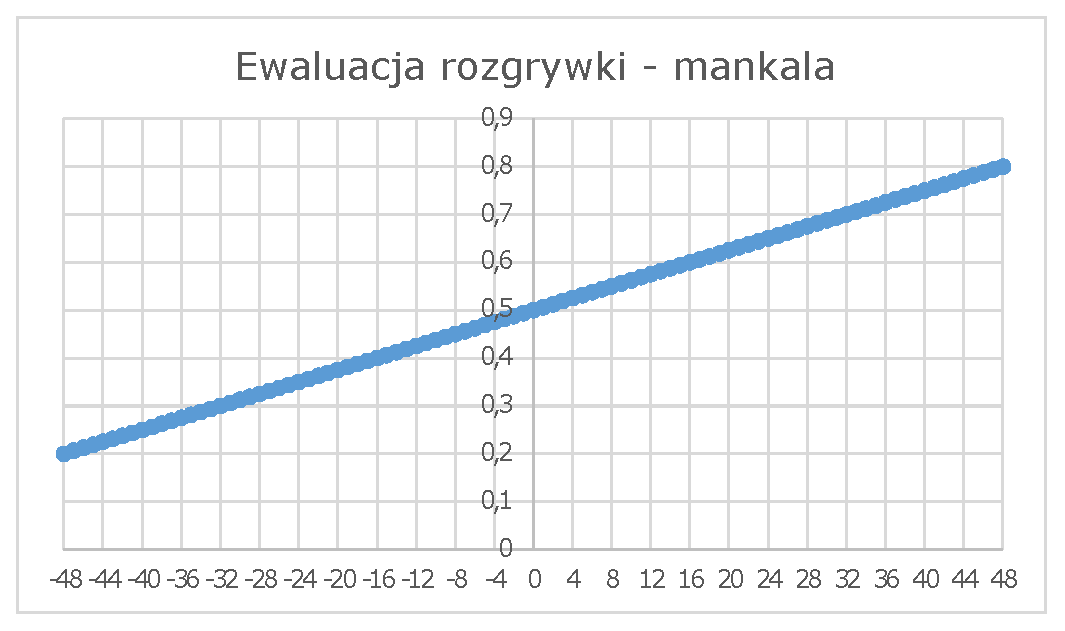
\includegraphics[width=0.7\linewidth]{wykres-mancala}
	\caption{Wykres funkcji nagrody dla mankali}
	\label{rys:eval_mancala}
\end{figure}

W przypadku szachów, podobnie jak w mankali, wartość nagrody jest zależna od różnicy materiału graczy. Różnicą względem rozwiązania ewaluacji w mankali jest rozróżnienie wartości figur. Przyjęte wartości zostały wymienione poniżej.

\begin{itemize}
	\item Pion -- $1$ punkt,
	\item Skoczek -- $3$ punkty,
	\item Goniec -- $3$ punkty,
	\item Wieża -- $5$ punków,
	\item Hetman -- $9$ punktów.
\end{itemize}

Oznacza to, że wartość początkowej kolekcji figur na szachownicy dla jednego gracza wynosi $39$ punktów. Maksymalna różnica punktów między graczami wynosić może zatem $39$ (lub więcej), zatem przyjęty przedział funkcji wyznaczającej wartość wypłaty dla gracza wynosi $[-39, 39]$. Dla różnicy wartości figur wynoszącej $0$ również przyjęto, że jest to wartość remisowa $0.5$.
Zamiast funkcji liniowej zdecydowano się na użycie funkcji $\arctan{x}$, której wartości w otoczeniu punktu przegięcia $x=0$ wraz ze wzrostem argumentów znacząco rosną, a wraz ze spadkiem -- znacząco maleją. Celem takiego zabiegu jest wypłacanie względnie wysokiej nagrody już dla małej różnicy w materiale (punktach) graczy.
Dokładny wzór funkcji przekształcający obraz funkcji $\arctan{x}$ na $[0.2, 0.8]$ prezentuje się następująco:
$$
f(x)=
0.3 \cdot \bigg[\arctan{\bigg(\frac{x}{4}\bigg) \cdot \frac{2}{\pi} + 1}\bigg] + 0.2
$$
a jej wykres znajduje się na Rysunku \ref{rys:eval_chess}.

\begin{figure}[h!]
	\centering
	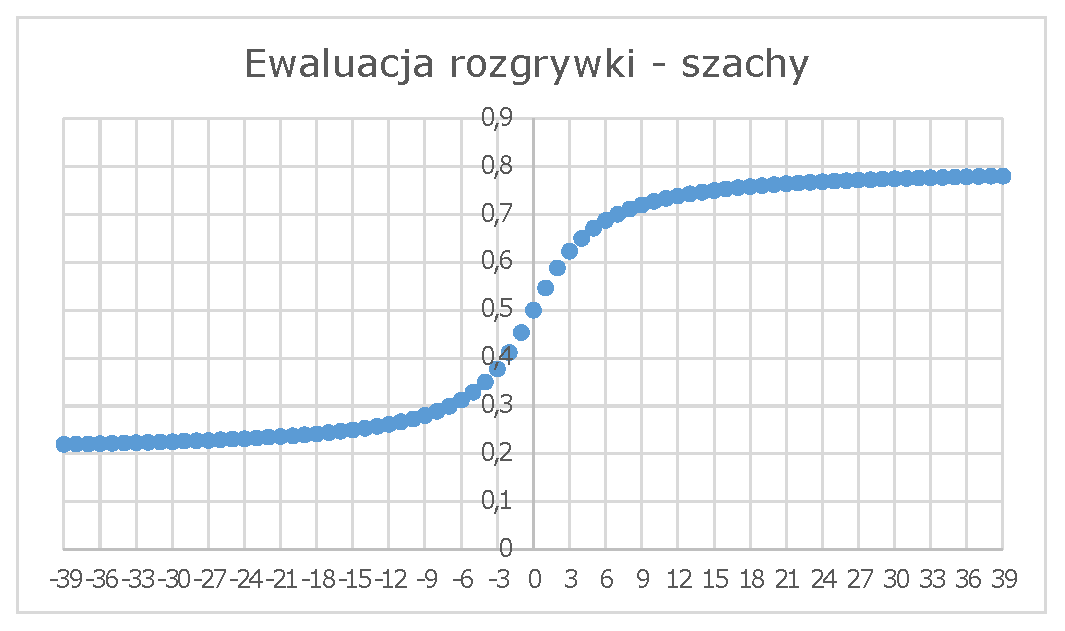
\includegraphics[width=0.7\linewidth]{wykres-szachy}
	\caption{Wykres funkcji nagrody dla szachów}
	\label{rys:eval_chess}
\end{figure}


\section{Moduł -- Serializacja} \label{subsec:serialization}
\textit{Serializacja} jest modułem odpowiadającym za zapisywanie drzew do plików formacie binarnym lub CSV. Pliki z drzewami w formacie binarnym mają umowne rozszerzenie \textit{.tree}. Oba schematy są rekurencyjne, ponieważ taka jest również struktura generowanych przez aplikację drzew. To oznacza, że w celu zapisania całego drzewa, wystarczy przekazać odpowiednim komponentom jego korzeń.


\section{Serializacja binarna}
W serializacji binarnej przyjmujemy opisany niżej schemat.

\begin{itemize}
	\item \textbf{liczba całkowita} -- wartość liczby zakodowanej w U2 z użyciem 4 bajtów. Bajty liczby w kolejności little endian.
	\item \textbf{napis} -- liczba bajtów w napisie \textit{(liczba całkowita)} i następnie zawartość napisu kodowana w UTF-8.
	\item \textbf{liczba zmiennoprzecinkowa} -- wartość liczby zakodowanej w IEEE754 z użyciem 64 bitów w kolejności little endian.
\end{itemize}

Schemat serializowania wierzchołka wykorzystuje wymienione powyżej zasady i ma następującą strukturę:

\begin{itemize}
	\item nazwa stanu \textit{(napis)},
	\item $m$ -- liczba węzłów potomnych \textit{(liczba całkowita)},
	\item $m$ powtórzeń następującego bytu:
	\begin{itemize}
		\item nazwa ruchu \textit{(napis)},
		\item licznik odwiedzin \textit{(liczba całkowita)},
		\item dodatkowy licznik odwiedzin \textit{(liczba całkowita)},
		\item średnia wypłata \textit{(liczba zmiennoprzecinkowa)},
		\item węzeł potomny \textit{(wierzchołek)}.
	\end{itemize}
\end{itemize}

\section{Serializacja do plików csv}
W serializacji do plików CSV przyjmujemy, że każdy kolejny wiersz odpowiada kolejnemu wierzchołkowi drzewa, a kolejne wartości opisujące wierzchołek oddzielamy przecinkami. Ostatnią wartością jest liczba wierzchołków potomnych. Każdy wierzchołek serializujemy do wiersza postaci:

\begin{center}
	\textbf{R, O, O2, W, S, D}
\end{center}
Oznaczenia:
\begin{itemize}
	\item R -- nazwa ruchu,
	\item O -- licznik odwiedzin,
	\item O2 -- dodatkowy licznik odwiedzin,
	\item W -- średnia wypłata algorytmu za ruch,
	\item S -- nawa stanu,
	\item D -- liczba wierzchołków potomnych.
\end{itemize}

Kolejność wierszy opisujących wierzchołki jest analogiczna do odwiedzania wierzchołków przez algorytm przeszukiwania drzewa wgłąb, począwszy od korzenia.

\begin{itemize}
	\item Jeśli wierzchołek $v$ ma jednego potomka $v_1$, to wiersz opisujący $v_1$ znajduje się pod wierszem opisującym $v$.
	\item Jeśli wierzchołek $v$ ma $n$ potomków $v_1, v_2, ..., v_n$ i żaden z potomków nie ma swoich potomków, to pod wierszem opisującym $v$ kolejne $n$ wierszy opisuje wierzchołki $v_1, v_2, ..., v_n$.
\end{itemize}


\section{Moduł -- Wizualizacja}
Moduł \textit{Wizualizacja} udostępnia funkcjonalność wyświetlania dostarczonych drzew. \textit{Wizualizacja} jest jedynym modułem, który korzysta z technologii \textit{VisPy} oraz \textit{NumPy}. Wykorzystanie tych technologii ma na celu odpowiednio wydajne wyświetlenie wizualizacji oraz przechowywanie wektorów z danymi, które będzie można przekazać procesorowi graficznemu. Zadania \textit{Wizualizacji} są wymienione poniżej.

\begin{itemize}
	\item Przypisanie wierzchołkom drzewa miejsca na płaszczyźnie przy użyciu usprawnionego algorytmu Walkera i przetransformowanie wyznaczonych współrzędnych do układu współrzędnych OpenGL.
	\item Przypisanie krawędziom koloru w zależności od liczby odwiedzin wierzchołka.
	\item Przypisanie wierzchołkom odpowiedniego koloru. W pracy przyjęto, że jeśli w stanie gry reprezentowanym przez wierzchołek podejmuje decyzję pierwszy gracz, to wierzchołkowi zostanie przypisany kolor biały. Natomiast jeśli wierzchołek będzie odpowiadał stanowi, w którym następuje ruch gracza drugiego, wierzchołkowi zostanie przypisany kolor czarny.
	\item Detekcja kliknięcia wierzchołka przez użytkownika.
	\item Wyświetlenie drzewa.
	\item Przybliżanie, oddalanie i poruszanie się po wizualizacji.
\end{itemize}


\section{Moduł -- Gry}
Prezentowane rozwiązanie udostępnia dwie gry planszowe w ramach modułu \textit{Gry}. System został przygotowany z myślą o rozszerzaniu o kolejne gry. Wymagania, które należy spełnić, dodając kolejną grę, są opisane w rozdziale \ref{subsec:uml}.

\subsection{Zasady gry w mankalę}
Mankala, jako jedna z przykładowych gier modułu \textit{Gry}, jest mniej popularną grą logiczną od szachów, więc postanowiono przedstawić instrukcję rozgrywki.\\

Plansza mankali, ukazana na schemacie na Rysunku \ref{rys:mancala}, zawiera dwanaście mniejszych pól i dwa większe, nazywane domami lub bazami. Każdemu z graczy przypisane jest sześć mniejszych pól leżących przed nim i dom po jego prawej stronie. Na początku gry w każdym z pól znajdują się cztery kamienie. Celem obu graczy jest zebranie jak największej liczby kamieni w ich domach. Gra kończy się, gdy wszystkie pola jednego z graczy są puste -- wtedy pozostałe kamienie przydzielane są drugiemu graczowi.\\

\begin{figure}[h!]
	\centering
	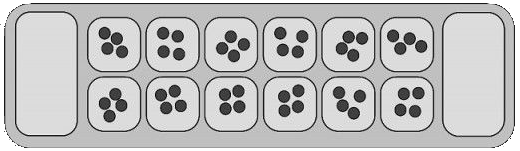
\includegraphics[width=0.6\textwidth]{mancala.png}
	\caption{Plansza mankali}
	\label{rys:mancala}
\end{figure}

Ruch gracza polega na wyjęciu wszystkich kamieni z wybranego własnego pola i rozdysponowaniu po jednym do kolejnych pól, omijając dom przeciwnika. Rozdysponowanie jest wykonywane w kierunku odwrotnym do ruchu wskazówek zegara. Ponadto, jeśli ostatni kamień wyląduje we własnym domu -- gracz musi wykonać kolejny ruch. W przeciwnym przypadku -- następuje ruch przeciwnika.\\

Ostatnią zasadą mankali jest bicie. Bicie następuje, jeśli po wykonaniu ruchu, ostatni kamień wyląduje na pustym polu gracza. W takiej sytuacji gracz zabiera wszystkie kamienie z przeciwległego pola planszy. Jeżeli w sąsiednim polu nie ma kamieni, nie dochodzi do ich przejęcia. Tak samo, ruch nie kończy się biciem, jeżeli ostatni kamień wyląduje na pustym polu przeciwnika.


\section{Moduł -- Aplikacja główna} \label{subsec:mainapp}
\textit{Aplikacja główna} jest modułem łączącym wszystkie pozostałe. Ten moduł skupia się na zaprezentowaniu funkcjonalności wszystkich modułów w formie aplikacji okienkowej. Interfejsy graficzne, które udostępnia \textit{Aplikacja główna}, są opisane w rozdziale \ref{sec:ui}.




